\chapter{总体设计}
\section{软件描述}
系统包括前台和后台两个部分。

前台主要功能是:
给用户提供交互的接口,用于各种功能。
后台主要功能是:
处理用户发出的请求,后台记录用户产生的数据等等。

\section{处理流程}
\subsection{总体流程}

\subsection{系统基本流程}
此处应当有一个图和对应的描述。

\subsection{客户端基本流程}
\begin{figure}[ht]
	\centering
	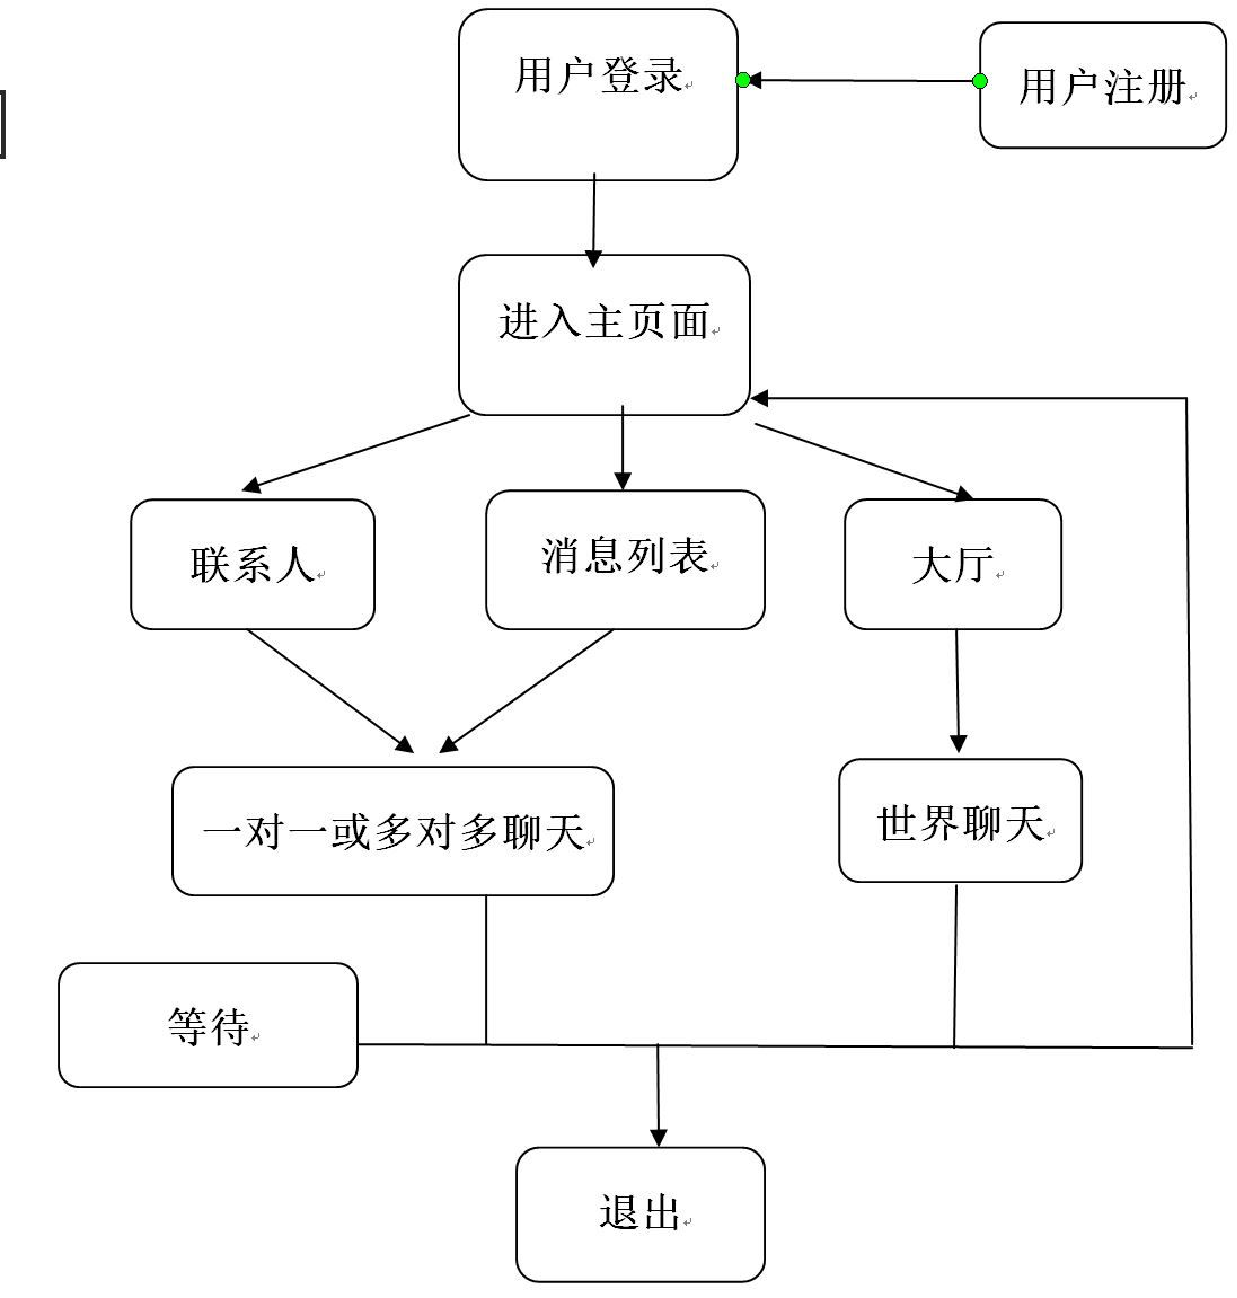
\includegraphics[width=10cm]{client}
	\caption{客户端流程} \label{fig:figure1}
\end{figure}


\subsection{服务器端基本流程}


\subsection{功能1具体流程}

用户注册或登录

在打开应用的第一个页面,会有用户名和密码的输入框,在正确输入用户名和密码之后点击sign in便可以登入。或者可以点击另外一个sign up的按钮,
创建一个用户名没有重复的账户之后输入验证码便会通过,服务器数据更新之后便可以使用这个新的账户登录。


\subsection{功能2具体流程}

单人聊天

已登录用户会进入一个新的功能页面(称为主页面)。在主页面首先在消息列表中选择的已有对话,或者在联系人列表中选择联系人新建对话。

\subsection{功能3具体流程}

大厅聊天

已登录用户在主页面选择大厅聊天,输入任何自己想说的并发送即可。要注意的是,在大厅说的所有话都会被所有在线用户看到。



\section{功能结构设计}
\subsection{整体结构}
此处应当有一个图和对应的描述。系统如果像微内核那样,划分成核心模块和若干个子系统,此处应当有图示及说明,然后后续几个节应当描述这几个子系统。如果系统像宏内核,那应当说明有哪些紧密联系的模块,并在后续几个节内描述这些模块。

\subsection{用户端结构}
此处应当有一个图和对应的描述。这只是举个例子。可能的内容包括用户端的具体模块、耦合情况等。

\subsection{服务器端结构}
此处应当有一个图和对应的描述。这只是举个例子。

\subsection{后台数据库维护模块结构}
此处应当有一个图和对应的描述。这只是举个例子。



\section{功能需求与程序代码的关系}
[此处指的是不同的需求分配到哪些模块去实现。可按不同的端拆分此表]
\begin{table}[htbp]
\centering
\caption{功能需求与程序代码的关系表} \label{tab:requirement-module}
\begin{tabular}{|c|c|c|c|}
    \hline
    · & LoginActicity.java & FragmentPeople.java & MessageActivity.java \\
    \hline
    用户注册 & Y & · & · \\
    \hline
    用户登录 & Y & · & · \\
    \hline
    连接服务器 & Y & · & · \\
    \hline
    文字聊天 & · & · & Y \\
    \hline
    添加删除联系人 & · & Y & · \\
    \hline
\end{tabular}
\note{各项功能需求的实现与各个程序模块的分配关系}
\end{table}